%Notes by Harsh Mistry 
%Econ 301
%Based on Template From  https://www.cs.cmu.edu/~ggordon/10725-F12/template.tex

\documentclass[twoside]{article}
\setlength{\oddsidemargin}{0.25 in}
\setlength{\evensidemargin}{-0.25 in}
\setlength{\topmargin}{-0.6 in}
\setlength{\textwidth}{6.5 in}
\setlength{\textheight}{8.5 in}
\setlength{\headsep}{0.75 in}
\setlength{\parindent}{0 in}
\setlength{\parskip}{0.1 in}
\usepackage{amsmath,amsfonts,graphicx, color}
\newcounter{lecnum}
\renewcommand{\thepage}{\thelecnum-\arabic{page}}
\renewcommand{\thesection}{\thelecnum.\arabic{section}}
\renewcommand{\theequation}{\thelecnum.\arabic{equation}}
\renewcommand{\thefigure}{\thelecnum.\arabic{figure}}
\renewcommand{\thetable}{\thelecnum.\arabic{table}}
\newcommand{\lecture}[4]{
   \pagestyle{myheadings}
   \thispagestyle{plain}
   \newpage
   \setcounter{lecnum}{#1}
   \setcounter{page}{1}
   
   
%Info Box 
   \begin{center}
   \framebox{
      \vbox{\vspace{2mm}
    \hbox to 6.28in { {\bf Econ 301 - Microeconomic Theory 2
	\hfill Winter 2018} }
       \vspace{4mm}
       \hbox to 6.28in { {\Large \hfill Lecture #1: #2  \hfill} }
       \vspace{2mm}
       \hbox to 6.28in { {\it Lecturer: #3 \hfill Notes By: #4} }
      \vspace{2mm}}
   }
   \end{center}
   
   \markboth{Lecture #1: #2}{Lecture #1: #2}



 
}

\renewcommand{\cite}[1]{[#1]}
\def\beginrefs{\begin{list}%
        {[\arabic{equation}]}{\usecounter{equation}
         \setlength{\leftmargin}{2.0truecm}\setlength{\labelsep}{0.4truecm}%
         \setlength{\labelwidth}{1.6truecm}}}
\def\endrefs{\end{list}}
\def\bibentry#1{\item[\hbox{[#1]}]}

\newcommand{\fig}[3]{
			\vspace{#2}
			\begin{center}
			Figure \thelecnum.#1:~#3
			\end{center}
	}
	
	\graphicspath{ {images/} }

\newtheorem{theorem}{Theorem}[lecnum]
\newtheorem{lemma}[theorem]{Lemma}
\newtheorem{ex}[theorem]{Example}
\newtheorem{proposition}[theorem]{Proposition}
\newtheorem{claim}[theorem]{Claim}
\newtheorem{corollary}[theorem]{Corollary}
\newtheorem{definition}[theorem]{Definition}
\newenvironment{proof}{{\bf Proof:}}{\hfill\rule{2mm}{2mm}}
\newcommand\E{\mathbb{E}}


%Start of Document 
\begin{document}

\lecture{12}{February 14, 2018}{Jean Guillaume Forand}{Harsh Mistry}

\section{Competitive Equilibrium Continued}
\begin{ex} Competitive equilibria need not exist. Let \(\omega^A = (1, 1) = \omega^B\), \(u^A(x^A_1, x^A_2) = \max \{x_1^A, x_2^A\}\) and \(u^B(x_1^B, x_2^B) =  x_1^{B \frac{1}{2}} x^{B \frac{1}{2}}_2\)
\begin{center}
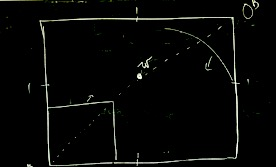
\includegraphics[scale=0.5]{18}
\end{center}
\begin{itemize}
\item Demand Function for A 
\[(x_1^A (p_1 \omega^A), x_2^A (p_1 \omega^A)) = \begin{cases}
\left( \frac{p_1 + p_2}{p_1} , 0 \right) & \text{ if } \frac{p_1}{p_2}  < 1\\
\left(\frac{p_1 +  p_2}{p_1}\right) \text { or}  \left(0, \frac{p_1 + p_2}{p_2} \right) & \text{ if } \frac{p_1}{p_2} = 1 \\
\left(0, \frac{p_1 + p_2}{p_2} \right) & \text{ if } \frac{p_1}{p_2} > 1
\end{cases}\]
\item Demand Function for B 
\[(x_1^B (p_1 \omega^B), x_2^B (p_1 \omega^B)) = \left(\frac{p_1 + p_2}{2p_1} , \frac{p_1 + p_2}{2p_2} \right)\]
\item Case 1 : Can  a competitive equilibrium have \(p_1^* = 0\) ? No, \(x_1^B (p_1^* \omega^B) \) is undefined if \(p_1^* = 0\)
\item Case 2 : Can we have a competitive equilibrium  with \(\frac{p_1^*}{p_2^*} < 1 \) ? No, (MC2) fails
\[\begin{aligned}x^B (p_1^* \omega^B)  = \frac{p_1^*+p_2^*}{2p_2}  &  = \frac{1}{2} \frac{p_1^*}{p_2^*} + \frac{1}{2} < 1  \\
& = \omega^A_2 + \omega^B_2 \end{aligned}\]
\item Case 3 : A similar argument shows that no competitive equilibrium with \(\frac{p_1^*}{p_2^*} > 1\) exists
\item Case 4 : Can we have a competitive equilibrium with \(\frac{p_1^*}{p_2^*} = 1\)? No, A demands 2 units if \underline{some} good B demands 1 unit of each good
\item \textbf{Therefore, some consumers don't meet equilibrium}
\end{itemize}
\end{ex}

\section{Welfare}
\textcolor{red}{In-Class Numbering : 3.0}
\begin{itemize}
\item So far, we have studied \underline{positive}, or descriptive properties of competitive equilibriums (i.e do they exists, how do prices vary with endowments,preferences, etc) 
\item Given this, our goal is to study \underline{normative} properties of competitive equilibrium (i.e which depend on value judgement) 
\begin{itemize}
\item How well do markets perform in allocating goods across consumers?
\item How do they compare against alternative exchange mechanisms?
\item We need to develop normative criteria to evaluate the performance of markets and/or other mechanisms. 
\end{itemize}
\item What would \underline{bargaining} between consumers look like? 
\begin{itemize}
\item Consider a two consumer economy 
\begin{center}
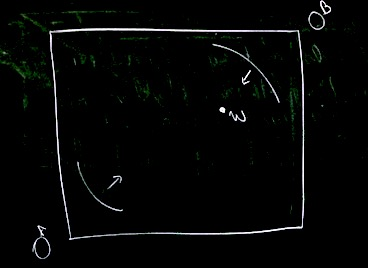
\includegraphics[scale=0.4]{19}
\end{center}
\item Bargaining protocols can be varied and complex, as a result we focus on describing allocations that are consistent with some bargaining process. 
\begin{center}
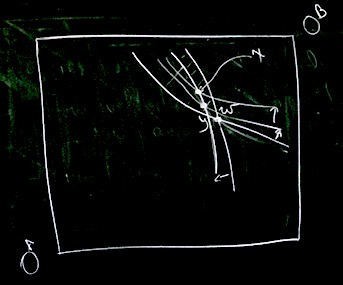
\includegraphics[scale=0.4]{20}
\end{center}
\item Any bargained agreement must deliver allocation \(x^J\) to consumer \(J = AB\) such that 
\[u^J(x_1^J, x_2^J) \geq u^J(\omega^J_1, \omega^J_2)\]
\item Any bargained agreement must be \underline{feasible}
\[x_i^A + x_i^B \leq \omega^A_1 + \omega^B_2 \text{ for } i = 1,2  \text{ (with equality if preferences are monotone)} \]
\item Are all feasible and individually rational allocations candidate bargained agreements? No, such allocations can be c  to mutually beneficial counterproposal
\end{itemize}
\end{itemize}
\begin{center}
\textbf{To be continued next lecture with examples}
\end{center}
\end{document}





